\chapter{Prima istanziazione}
\section{Schema a blocchi e definizione dei segnali IN/OUT:}
In base a quanto detto nel precedente capitolo si può procedere ad una prima istanziazione della CPU.
\begin{figure}[H]
	\centering
	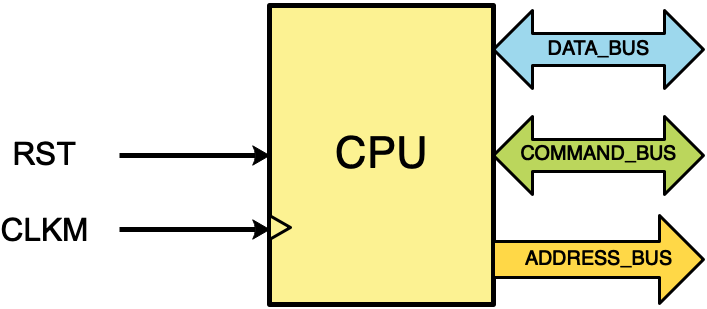
\includegraphics[scale=0.5]{1_prima_istanziazione}
	%\caption{Gesione della memoria in un'architettura di Von Neumann migliorata}
	\label{fig:prima_istanziazione}
\end{figure}
I segnali presenti a questo livello sono:
\begin{itemize}
	\item \textbf{OPERANDI E RISULTATO:}
	\begin{itemize}
		\item \textbf{DATA\_BUS} (N bit): bus dati di input-output connesso con il bus DATI di sistema.
		\item \textbf{COMMAND\_BUS} (N bit): bus contenente un raggruppamento dei segnali di controllo connesso con il bus COMANDI di sistema.
		\item \textbf{ADDRESS\_BUS} (2N bit): bus contenente i segnali di indirizzo per la memoria e le periferiche, connesso con il bus INDIRIZZI di sistema.
	\end{itemize}
	
	\item \textbf{CLOCK MACCHINA:}
	\begin{itemize}
		\item \textbf{CLKM}: clock macchina per evoluzione sincrona.
	\end{itemize}
	
	\item \textbf{RESET:}
	\begin{itemize}
		\item \textbf{RST}: \{0: funzionamento normale; 1: reset attivo $\rightarrow$ il sistema riavvia l'esecuzione dalla prima istruzione\}.
	\end{itemize}
\end{itemize}

\section{Regola protocollare:}
\begin{itemize}
	\item \textit{ESTERNO}:
	\begin{enumerate}
		\item La macchina procede con l'esecuzione del programma salvato nella memoria RAM in modo sequenziale evolvendo con gli impulsi di clock esterni.
	\end{enumerate}

	\item \textit{INTERNO}:
	La CPU si trova nella condizione di reset e genera l'indirizzo 0000h per la memoria. Tale locazione conterrà la prima istruzione del programma scritto in RAM. Per ogni istruzione si esegue il ciclo di fetch-execute:
	\begin{enumerate}
		\item FETCH: La CPU preleva l'istruzione dalla memoria all'indirizzo fornito dal PC e la salva nel registro istruzione IR. Infine esegue un aggiornamento del PC.
		\item DECODE: La CPU riconosce l'istruzione e si occupa del prelievo eventuale dei dati dalla memoria salvandoli nei registri di appoggio interno.
		\item EXECUTE: La CPU esegue l'istruzione.
		\item (se previsto) WRITE-BACK: La CPU si occupa del salvataggio del dato sulla memoria.
	\end{enumerate}
\end{itemize}

\section {Task eseguibili, set di istruzioni e organizzazione della RAM interna:}
In questa sezione ci si occupa di definire parte del set di istruzioni relativo a quanto discusso nel paragrafo \textquotedblleft Metodi di indirizzamento" di pagina \pageref{metodi_di_indirizzamento}. Riassumendo i task da eseguire e considerando i dati relativi a tali istruzioni si ottiene la seguente tabella.
\begin{table}[H]
	\centering
	\footnotesize
	\fontsize{10}{18}\selectfont
	\begin{tabular}{|p{0.5cm}|p{0.5cm}|p{0.5cm}|p{0.5cm}|p{0.5cm}|p{0.5cm}|}
		\hline
		\multicolumn{1}{|c|}{\textbf{INSTRUCTION}} & \multicolumn{1}{c|}{\textbf{CODE}} & 
		\multicolumn{3}{c|}{\textbf{BINARY EQUIVALENT}} & \multicolumn{1}{l|}{\textbf{MODIFIERS}} \\
		
		& & \multicolumn{1}{|c|}{COD. OP}  & \multicolumn{1}{|c|}{1st nibble} & \multicolumn{1}{|c|}{2nd nibble} & 	 \\ \hline
		
		\multicolumn{1}{|l|}{No operation}	&
		\multicolumn{1}{|c|}{NOP}  &
		\multicolumn{1}{|c|}{0000}	&
		\multicolumn{1}{|c|}{-} &
		\multicolumn{1}{|c|}{-} &
%		\multicolumn{1}{|c|}{-} &
		\multicolumn{1}{|c|}{-}	\\ \hline
		
		
		\multicolumn{1}{|l|}{Read RAM}	&
		\multicolumn{1}{|c|}{RD}  &
		\multicolumn{1}{|c|}{0001}	&
		\multicolumn{1}{|c|}{$A_7A_6A_5A_4$} &
		\multicolumn{1}{|c|}{$A_3A_2A_1A_0$} &
%		\multicolumn{1}{|c|}{-} &
		\multicolumn{1}{|l|}{address}	\\ \hline
		
		\multicolumn{1}{|l|}{Write RAM at address}	&
		\multicolumn{1}{|c|}{WR}  &
		\multicolumn{1}{|c|}{0011}	&
		\multicolumn{1}{|c|}{$A_7A_6A_5A_4$} &
		\multicolumn{1}{|c|}{$A_3A_2A_1A_0$} &
%		\multicolumn{1}{|c|}{$D_3D_2D_1D_0$} &	
		\multicolumn{1}{|l|}{address, data}	\\ \hline
		
		\multicolumn{1}{|l|}{Jump at Address}	&
		\multicolumn{1}{|c|}{JPA}  &
		\multicolumn{1}{|c|}{0100}	&
		\multicolumn{1}{|c|}{$A_7A_6A_5A_4$} &
		\multicolumn{1}{|c|}{$A_3A_2A_1A_0$} &
%		\multicolumn{1}{|c|}{-} &
		\multicolumn{1}{|l|}{address}	\\ \hline
		
		\multicolumn{1}{|l|}{Jump Offset}	&
		\multicolumn{1}{|c|}{JPO}  &
		\multicolumn{1}{|c|}{0101}	&
		\multicolumn{1}{|c|}{$O_3O_2O_1O_0$} &
		\multicolumn{1}{|c|}{-} &
%		\multicolumn{1}{|c|}{-} &
		\multicolumn{1}{|l|}{offset}	\\ \hline
		
		\multicolumn{1}{|l|}{Jump at Base+Offset}	&
		\multicolumn{1}{|c|}{JBO}  &
		\multicolumn{1}{|c|}{0111}	&
		\multicolumn{1}{|c|}{$B_3B_2B_1B_0$} &
		\multicolumn{1}{|c|}{$O_3O_2O_1O_0$} &
%		\multicolumn{1}{|c|}{-} &
		\multicolumn{1}{|l|}{base, offset}	\\ \hline
		
		\multicolumn{1}{|l|}{Move reg A to B}	&
		\multicolumn{1}{|c|}{MV}  &
		\multicolumn{1}{|c|}{1000}	&
		\multicolumn{1}{|c|}{$A_3A_2A_1A_0$} &
		\multicolumn{1}{|c|}{$B_3B_2B_1B_0$} &
%		\multicolumn{1}{|c|}{-} &
		\multicolumn{1}{|l|}{reg. A, reg. B}	\\ \hline
	\end{tabular}
	\caption{Set di istruzioni}
\end{table} 		
\noindent
Il numero di bit riservato al codice operazione è sovradimensionato rispetto al numero di operazioni. Per discriminare tra le operazioni possibili sarebbero stati sufficienti $\lceil log_2{7} \rceil = 3$ bit; tuttavia considerando la futura ed eventuale aggiunta di ulteriori istruzioni, nonchè il fatto di avere un bus dati a 4 bit, si è scelto di mantenere un codice operazione a 4 bit.\\
Come si può notare dalla tabella precedente sistema lavora su istruzioni operanti su 0, 1, o 2operandi a 4 bit. Sarà dunque compito della UC interna, una volta prelevata l'istruzione ed eseguita la decodifica, richiedere il numero di dati necessari all'esecuzione dell'istruzione stessa.
\par \bigskip \noindent
Si ricorda che la memoria è organizzata come in Figura \ref{fig:vn_mem}, dunque le istruzioni del programma troveranno posto in modo sequenziale nell'area \textquotedblleft istruzioni", così come i dati nell'area \textquotedblleft dati" sottostante. 
Poiché si dispone di un bus dati a 4 bit, nelle istruzioni dove si debba prelevare un indirizzo dalla memoria, si necessita di più accessi a locazioni di memoria contigue presenti all'area dati.
Si suppone dunque che la fase di traduzione da codice assembler a linguaggio macchina tenga conto di tale questione, procedendo ad inserire i dati nell'area di memoria dedicata ordinati in maniera sequenziale.

\section{Strategia e problematiche}
La struttura interna della CPU sarà ricavata in questo paragrafo tenendo conto del set di istruzioni e delle prerogative di progetto.\\
Anzitutto poiché dati e programmi sono reperiti a runtime dalla memoria RAM interna sarà necessario dotare la CPU di sistemi che permettano l'indirizzamento della memoria ai programmi ed al dato. In particolare si necessiterà quindi di due puntatori: un \textquotedblleft program counter" ed un \textquotedblleft data counter". Il PC conterrà l'indirizzo relativo alla prossima istruzione da eseguire, mentre il DC contiene l'indirizzo relativo al dato da prelevare.
In generale si può considerare che l'indirizzo per la lettura/scrittura della memoria può avere due sorgenti:
\begin{itemize}
	\item il PC: come nel caso del prelievo delle istruzioni.
	\item il DC: come nel caso del prelievo/scrittura dei dati.
\end{itemize}
A tal proposito, nel procedere al corretto indirizzamento della memoria, l'uscita del bus indirizzi sarà pilotata da un registro al cui ingresso è presente un multiplexer controllato dalla UC interna col fine di discriminare quale dei due registri sorgenti contenga il valore di indirizzo corretto.\\
Entrambi i registri PC e DC, devono essere aggiornati (incrementati di 1) ad ogni prelievo relativamente di un'istruzione o di un dato. A tal proposito si doteranno entrambi i registri della possibilità di auto-incremento affiancando agli stessi un sommatore semplice.
\par \bigskip \noindent
Nel caso dell'operazione di RD si vuole garantire la possibilità che l'indirizzo da fornire alla RAM per la lettura possa provenire da uno dei registri interni della CPU. Questo per fare in modo che l'indirizzo per la memoria possa essere generato internamente, ad esempio a seguito di un calcolo. A tal proposito si può pensare di inserire un particolare registro d'appoggio presente nel banco dei registri interni e denominato AR0 che possa pilotare direttamente il bus indirizzi. Il dato letto viene caricato sul registro bidirezionale in/out.
\par \bigskip \noindent
Nel caso delle operazione di WR, come nel caso della RD, l'indirizzo sul quale effettuare la scrittura proviene dal registro AR0 interno al banco d'appoggio della CPU. Si suppone che il dato da salvare sia già stato precaricato all'interno del registro bidirezionale in/out che pilota il bus dati dal lato CPU.
\par \bigskip \noindent
Nel caso della jump immediata l'indirizzo di salto è indicato dal valore del dato prelevato dalla memoria. Dunque si doterà il PC della possibilità di essere aggiornato al valore presente nel registro bidirezionale di ingresso/uscita, attraverso un mux di selezione.
\par \bigskip \noindent
Nel caso delle operazioni denominate JPO e JBO il risultato del salto è dato dalla somma di un indirizzo \textquotedblleft \textit{base}" e di un \textit{offset}. Dunque sarà utile dotare la CPU di una unità di calcolo ausiliare, in modo da non necessitare dell'impiego della ALU principale nel caso di calcolo di tali indirizzi di salto.
\par \bigskip \noindent
Infine, considerando la struttura elementare interna di un'architettura di Von Neumann come quella riportata in Figura \ref{fig:vn_cpu}, la CPU contiene al suo interno un banco di registri di appoggio al calcolo. In particolare, nel caso relativo a questo esercizio, oltre ai già noti PC e DC trovano posto:
\begin{itemize}
	\item 10 registri di appoggio per i dati con etichetta.
	\item 1 registro accumulatore ACC.
	\item 4 registri di supporto al calcolo di ADDR, tra cui AR0.
	\item 1 registro bidirezionale per il salvataggio dei dati in ingresso/uscita, connesso al bus dati di sistema.
\end{itemize}
Su tutti questi registri si applica l'operazione di move parametrica (COD. OP: MV), la quale eseguirà la copia del contenuto di uno dei registri sorgente in un altro di destinazione. Per l'esecuzione di tale operazione si può pensare di inserire all'interno dell'area dedicata ai registri una logica combinatoria che apra il \textquotedblleft canale di transito" al dato dal registro sorgente a quello destinazione. Uno strobe da parte della UC master sul registro destinazione ne copierà il dato all'interno completando l'operazione. Per discriminare i registri coinvolgibili in tale operazione si doterà ognuno di questi di una etichetta caratteristica, ossia definita a livello di microcodice. Al programmatore sarà sufficiente scrivere i tag dei registi opportuni nella programmazione a livello assembler per garantire la riuscita dell'operazione in modo corretto.
\par \bigskip \noindent
Detto questo si può procedere alla seconda istanziazione della CPU.